\chapter{Result}
\label{results}
Having a concept on how to translate a rust program into a Petri-Net, we can now inspect the actual results.
\section{Translation Target}
In figure \ref{function_call_net} we can see the generated net for the function call program \ref{function_call_program} from the last chapter (since this is small enough to show and big enough to not be trivial).
This is the true data that was produced for the dot target so we cannot immediately see the virtual boundaries for statements basic blocks and functions.
To make the structure more clear the nodes where rearranged so that the called function is on the left and the main function on the right.
The initialized places of the locals where renamed to show their name (locals are scoped by functions so their names are not unique).

We can see a path from program start to program end;
The panic place is unconnected because the program cannot panic.
Local life cycles are also visible as a single edged path from marked uninitialized place to unmarked dead places.
Variable manipulation always has parallel incoming and an outgoing edges.
On a closer look we can see that local $\_3$ of the called function has no initializing and uninitializing statements.
This is actually a correct representation of the MIR graph:
for some reason the storage statements are not generated for some lvalues (in this case the lvalue from checked multiplications).
If this is expected behavior is not known at the time of writing;
A bug report \cite has yet to be solved.
Unfortunately this behavior introduces an unintended deadlock into our translation since depending transitions can only fire if the initialized places where previously marked.
To use the net for verification we have to work around this issue until it is fixed (or until the cause is modeled correctly).
Te be able to continue testing simply all initialized place where marked.
This way the involved transitions can fire, but only if the previous transition produced a token on the connecting place (the program counter place). 
An additional taken will also remain on the initialized places even after the storage dead transition fired.
However execution flow, again, will not be affected because of the program counter places.

A second detail that the net shows is that the function call transition is implicit;
The last statement of the main functions first basic block is directly connected to the first statement of the callees first basic block.
This is an implementation detail of the translator.
Since our model currently always inlines function calls (it generates a separate net for every call), these are entirely sequential.
That means a missing transition does not harm.
If previously translated functions shall be reused though, this issue needs rework.
But to be able to skip inlining we need high level semantics anyway.

An additional issue that can come to attention is that the assert terminator has no cleanup path that could lead to a panic.
Logically the assert is inserted because the preceding checked multiplication can overflow which is undefined behavior and by default should panic in rust semantics.
This program actually cannot fail at this point since the involved variables are constant and small enough to be multiplied.
If this is the reason why the panic path is not generated (or optimized away) in the MIR representation however, shall be a question for the rust compiler team.


\begin{figure}
  \centering
  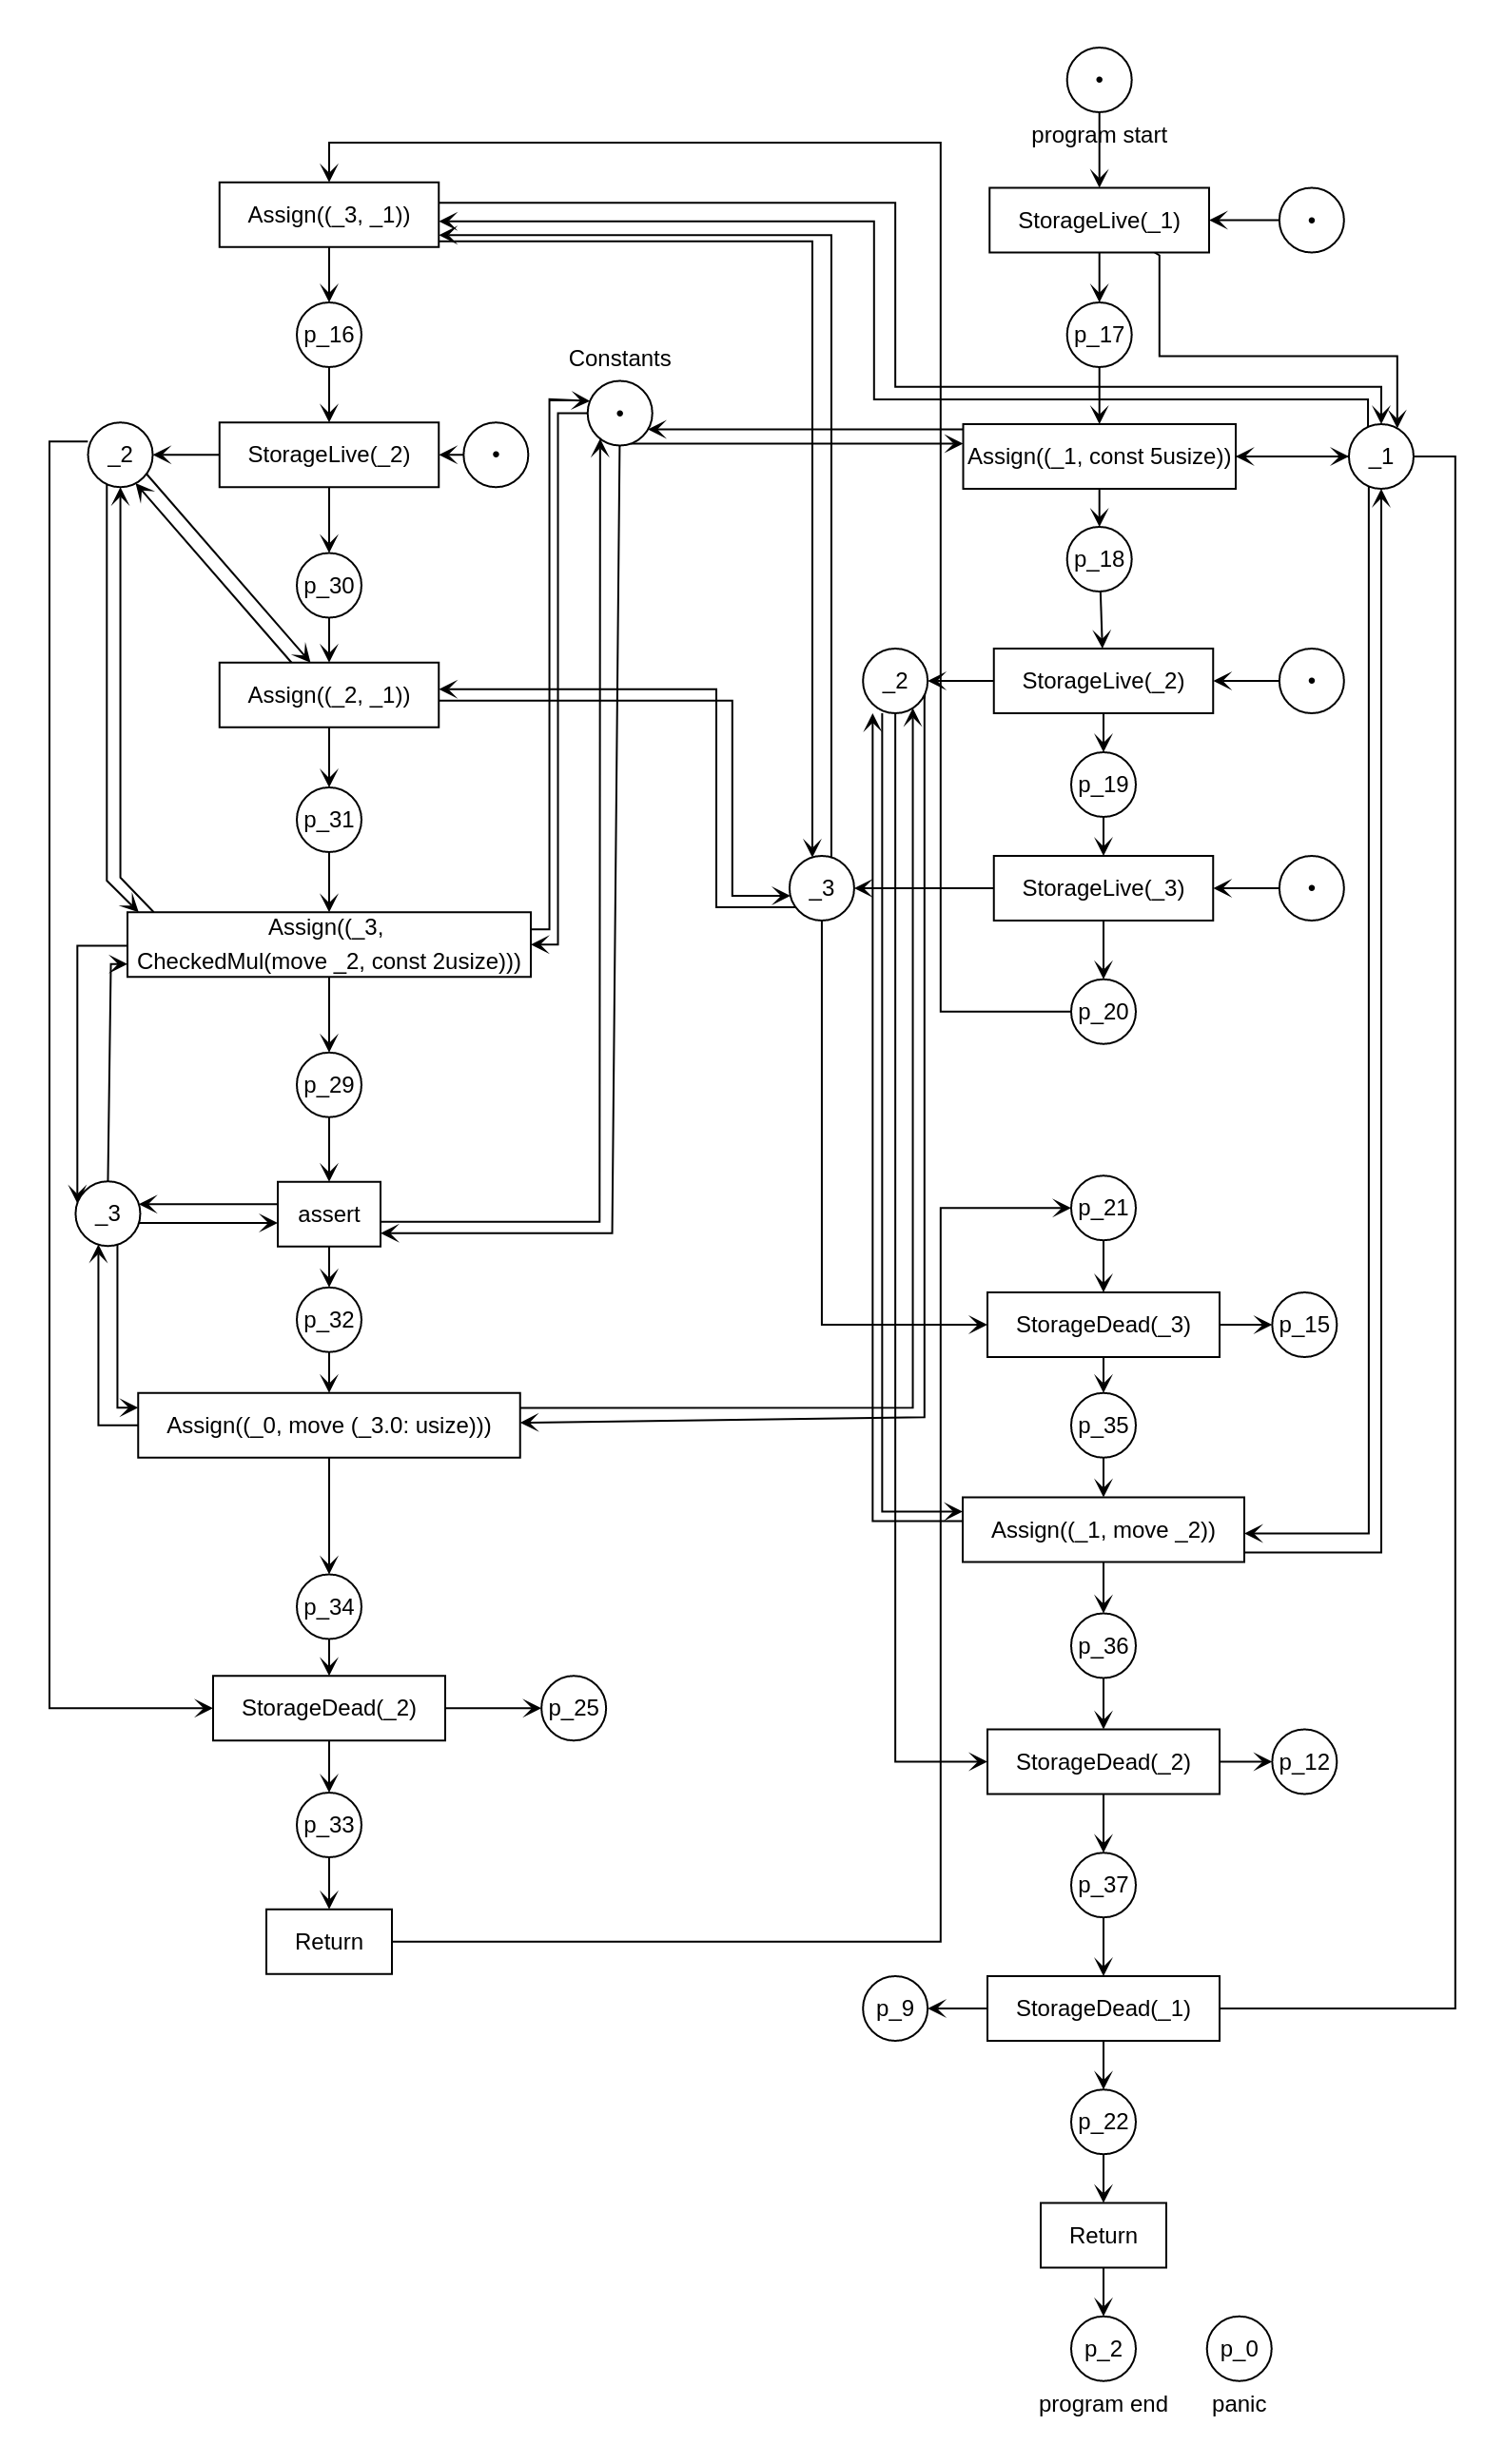
\includegraphics[width=0.9\textwidth]{../diagrams/FunctionCallNet.png}
  \caption{Translated Petr-net}
  \label{function_call_net}
\end{figure}
\begin{verbatim}
- expected deadlocks are detected (expected program termination)
- examples
  - minimal deadlock
    - detected with variable marking
    - not detected without emulation
\end{verbatim}

\section{Discussion}
\subsection{Analysis}
\begin{verbatim}
-  net is safe
-  without the use of some data even most flow related properties
   are not discoverable this makes emulation necessary
-  a new local <-> memory model makes sense
-  makes emulation easier but does not resolve the problem
-  high lvl nets might resolve this issue at an unknown performance cost
  - deadlock with multiple threads
    - dining philosophers
    - thread emulation not implemented
  - data dependent deadlock
\end{verbatim}
  
\subsection{Translation}

\begin{verbatim}
- how easy/mapping quality
    - flow is easy
    - data is difficult
        - data is moved between many locals
        - moving quickly masks semantic e.g. for mutexes
- rusts borrow checking rules can probably be exploited better
- foreign functions cannot be translated and must be emulated
    - special emulation makes sense for some of them
    - especially for flow relevant functions like threads and mutexes

\end{verbatim}

\subsection{Verification}
\begin{verbatim}
- data representation
- connectiveness of the graph
- possibility of panics can be detected
    - little usefulness in complex programs
- simple deadlocks can already be detected
    - finding a correct formula is not trivial
        - panic paths mask normal execution deadlocks
        - splitting paths can mask deadlocks from single paths
- more sophisticated approach is necessary
\end{verbatim}
